\usetikzlibrary{calc}
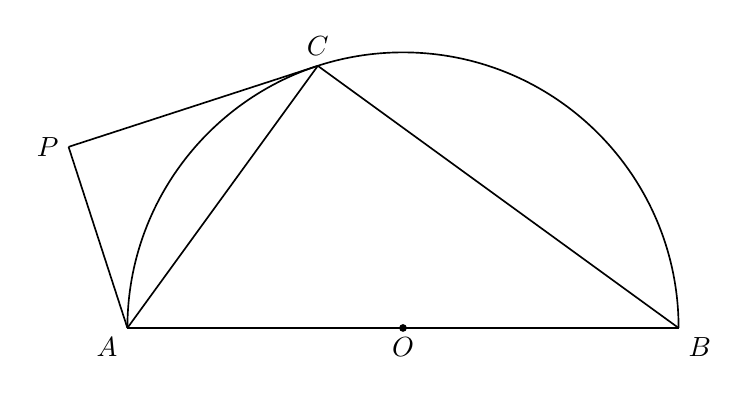
\begin{tikzpicture}[x=1cm,y=1cm,line width=.6pt,font=\normalsize]
\coordinate (A) at (-3.5,0);
\coordinate (B) at (3.5,0);
\coordinate (O) at (0,0);
\coordinate (C) at (-1.0815595,3.3286978);
\coordinate (P) at (-4.2473392,2.3000736);
\draw (A) arc[start angle=180,end angle=0,radius=3.5cm];
\draw (A)--(B);
\draw (A)--(C);
\draw (C)--(B);
\draw (A)--(P);
\draw (P)--(C);
\fill (O) circle[radius=1.4pt];
\node[below left] at (A) {$A$};
\node[below] at (O) {$O$};
\node[below right] at (B) {$B$};
\node[above] at (C) {$C$};
\node[left] at (P) {$P$};
\end{tikzpicture}
